\documentclass[12pt]{report}
\usepackage{graphicx}
% \usepackage[utf8]{vietnam}
\usepackage[left=3cm, right=3cm, top=3cm, bottom =3cm]{geometry}
\usepackage{pdfpages}
\usepackage{fancyhdr}
\usepackage{hyperref}
\usepackage{etoolbox}
\usepackage{float}
\usepackage{amsmath}

\usepackage[nottoc,notlof,notlot]{tocbibind} 
\renewcommand\bibname{References}

% \setcounter{tocdepth}{4}

% Link color setup
\hypersetup{
	colorlinks = true,
	linkcolor = black,
	citecolor = blue
}

% Change format of page
\pagestyle{fancy}
\fancyhf{}
\fancyhead{}
\fancyfoot{}
\fancyhead[L]{English}
\fancyfoot[L]{Ta Quang Tung}
\fancyfoot[R]{\thepage}
\renewcommand{\headrulewidth}{1pt}
\renewcommand{\footrulewidth}{1pt}

% \patchcmd{\chapter}{\thispagestyle{plain}}{\thispagestyle{fancy}}{}{}

\renewcommand{\thesection}{\arabic{section}}
\renewcommand{\thesubsection}{\thesection.\arabic{subsection}}
\renewcommand{\thesubsubsection}{\thesubsection.\arabic{subsubsection}}

% format
\usepackage{titlesec}
\usepackage{etoolbox}
\makeatletter
\patchcmd{\ttlh@hang}{\parindent\z@}{\parindent\z@\leavevmode}{}{}
\patchcmd{\ttlh@hang}{\noindent}{}{}{}
\makeatother

\titleformat{\subsection}
{\normalfont\large\bfseries}{\thesubsection}{1em}{}
\titleformat{\subsubsection}
{\normalfont\large\sffamily\bfseries}{\thesubsubsection}{1em}{}

% tab command
\newcommand\tab[1][1cm]{\hspace*{#1}}

\begin{document}

\begin{titlepage}

\newcommand{\HRule}{\rule{\linewidth}{0.5mm}} % Defines a new command for the horizontal lines, change thickness here

\center % Center everything on the page
 
%----------------------------------------------------------------------------------------
%   HEADING SECTIONS
%----------------------------------------------------------------------------------------

\textsc{\Large Hanoi University of Science and Technology}\\[1cm] % Name of your university/college
% \textsc{\LARGE INSTITUTE OF TECHNOLOGY  }\\[0.3cm]
% \textsc{\Large JALANDHAR-144011, PUNJAB(INDIA) }\\[0.3cm]
\textsc{\large English}\\[0.5cm] % Major heading such as course name
 % Minor heading such as course title

%----------------------------------------------------------------------------------------
%   TITLE SECTION
%----------------------------------------------------------------------------------------

\HRule \\[0.4cm]
{ \huge \bfseries Principles of Package Design}\\[0.03cm] % Title of your document
\HRule \\[1.5cm]

 
%----------------------------------------------------------------------------------------
%   AUTHOR SECTION
%----------------------------------------------------------------------------------------

\begin{minipage}{0.4\textwidth}
\begin{flushleft} \large
\emph{Student's Name:}\\
Ta Quang Tung
\end{flushleft}
\end{minipage}
~
\begin{minipage}{0.4\textwidth}
\begin{flushright} \large
\emph{Lecturer:} \\
Nguyen Thanh Hung
\end{flushright}
\end{minipage}\\[3cm]

% If you don't want a supervisor, uncomment the two lines below and remove the section above
%\Large \emph{Author:}\\
%John \textsc{Smith}\\[3cm] % Your name

%----------------------------------------------------------------------------------------
%   DATE SECTION
%----------------------------------------------------------------------------------------

{\large \today}\\[1cm] % Date, change the \today to a set date if you want to be precise

%----------------------------------------------------------------------------------------
%   LOGO SECTION
%----------------------------------------------------------------------------------------


\includegraphics[width=4cm]{hust.jpg}\\[1cm] % Include a department/university logo - this will require the graphicx package
 
%----------------------------------------------------------------------------------------

\vfill % Fill the rest of the page with whitespace

\end{titlepage}

\pagenumbering{gobble}
\tableofcontents 
\newpage

\pagenumbering{arabic}
\newpage
\setcounter{page}{1}

\section*{Introduction}
\addcontentsline{toc}{section}{Introduction}
As software application grow in size and complexity, 
they require some kind of high-level organization.
Classes, while a very convenient unit for organizing small application,
are not enough in large application. 
Something larger than class is needed.
That something is called a package. 

In UML, packages can be used as containers for groups of classes. 
By grouping classes into packages, 
we can reason about the design at a high level of abstraction,
higher than classes can do. 

We can also use the packages to manage the development 
and distribution of the software. 
The main goal is to partition the classes in an application according
to some criteria, and then allocate the classes 
in those paritions to packages. 

But classes often have dependencies on other classes,
and these dependencies will very often cross package boundaries. 
Thus, the packages will have dependency relationships with each other. 
The relationships between packages is 
high level organization of application,
and need to be managed.

We have large number of questions when allocating classes to packages.

For example:
\begin{itemize}
    \item What are the principles 
        for allocating classes to packages?
    \item What design principles govern the 
        relationships between packages?
    \item Should packages be designed before classes (top down)? 
        Or should be designed before packages (bottom up)?
    \item How are packages are physically represented? 
        In C++? In Java? In the development environment?
    \item Once created, what is the purpose will 
        we put these packages.
\end{itemize}

\section{Granularity: The Principles of Package Cohesion}
The three principles of package cohesion help developers decide how to parition classes into packages. 
They depend on the fact that least some of the classes 
and their interrelationships have been discovered. 
Thus, these principles take a "bottom-up" view of paritioning.

\subsection{The Reuse-Realese Equivalent Principle (REP)}

\tab \textit{The granule of reuse is granule of release}
\cite{reuse-release}

When you going to use another person's code, you want the author 
to guarantee to maintain it for you. 
After all, if you have to maintain it, you are going to have to invest
a tremendous amount of time into it -- time that might be better
spent designing a smaller and better package for yourself.

Second, you want the author to notify you any changes he plans to make 
to the interface and functionality of the code. 
But notification is not enough. The author must give you the option to 
refuse to use any new versions. 
After all, he might introduce a new version 
while you are not ready to accept it. It might be make changes to the code 
that are simply imcompatible with your system. 

In that case, you should decide to reject his version, the author
must guarantee to support your use of old version for a time. 
Perhaps that time is as short as three months or as long as a year. 
He can't just cut you loose and refuse to support you. If he won't agree to support your use of his old versions, then you may have to seriously consider whether you want to use his code.
In order to provide the guarantees that reusers need, authors must organize their software into reusable packages and then track those packages with release numbers.

The REP states that the granule of reuse 
can be no smaller than the granule of release. 
Any thing that reuse must also be released and tracked. 
It is not realistic for a developer to simply write a class and 
then claim it is reusable. 
Reusability comes only after there is a tracking system in place that offers the guarantees of 
notification, safety, and suport that the potential reusers will need. 

Reusable packages msut contain reusable classes. If a package contains software that 
should be reused, then it should not also contains software that is not designed for reuse. \textit{Either all of the classes in a package are reusable or none of them are}.

\subsection{The Common-Reuse Principle (CRP)}

\tab \textit{The classes in a package are reused together. If you reuse one of the classes in a package, you reuse them all.}

Classes are seldom reused in isolation. Generally, reusable classes 
collaborate with other classes that are part of 
the reusable abstraction. The CRP states that these classes belong together
in the same package. 
In such a package, we would expert to see classes that have lots of 
dependencies on each other.

A simple example might be a container class and its associated iterators. 
These classes are reused together
because they are tightly coupled to each other. 
Thus, they should to be in the same package.

But the CRP tells us more than just what 
classes to put together in a package. 
It also tell us what classes not to put in the package.
When on package uses another, a dependency is created between the packages.
It may be that using package only uses one class within the used package. 
However, that doesn't weaken the dependency at all. 
The using package still depends on the used package. 
Every time the used package is released, the using package must be validated and rereleased.
This is true event if the used package is being released because of changes to a class that the using package doesn't care about.

Moreover, it is common for packages to be compiled as shared libraries.
And then, when you use a package, you depend on the entire shared library.

Thus, it necessary to make sure that when I depend on a package, I depend on every class in that package. 
\subsection{The Common-Closure Principle (CCP)}

\tab \textit{The classes in a package should be closed together 
against the same kinds of changes. 
A change that affects a package affects all 
the classes in that package and no other packages.} \cite{Granularity}

This is the Single-Responsibility Principle 
restated for packages. 
Just as the SRP says that a class should not 
contain multiples reasons to change, 
this principle says that a package should not 
have multiple reasons to change.

In most applications, maintainability is more important that reusability. 
If the code in an application must
change, you would rather that the changes occur 
all in one package, rather than being distributed through many
packages. If changes are focused into a single package, 
then we need only release the one changed package. 
Other packages that don't depend on the changed package 
do not need to be revalidated or rereleased.

The CCP prompts us to gather together in one place all the classes that are likely to change for the same 
reasons. If two classes are so tightly bound, either physically or conceptually, that they always change together, then
they belong in the same package. This minimizes the workload related to releasing, revalidating, and redistributing
the software.

This principle is closely associated with the Open-Closed Principle (OCP). 
For it is "closure" in the OCP sense of the word 
this principle is dealing with. 
The OCP states that classes should be closed for modification
but open for extension. But 100\% closure is not attainable. 
Closure must be strategic. We design our systems such that 
they are closed to the most common kinds of changes 
that we have experienced.

The CCP amplifies this by grouping together classes 
that are open to certain types of changes into the same packages. 
Thus, when a change in requirements comes along, 
that change has a good chance of being restricted to
a minimal number of packages.

\section{Stability: The Principles of Package Coupling}
The next three principles deal with the relationships between
packages. Here again, we will run into the tension between
developability and logical design.

\subsection{The Acyclic-Dependencies Principle (ADP)}

\tab\textit{Allow no cycles in the package-dependency graph.}

\subsubsection{The "morning-after syndrome"}
When you are working at some large project, where many developers are 
modifying the same source files. 
You may encounter "morning-after syndrome". 
It happens when you maked some stuff working, went to home, 
arrive next moring and find out your stuff no longer works.
Because somebody stayed later than you changed something you depend on.

In small project, it isn't a big problem. 
But as the size of project grows, it can become a nightmare.
Everyone keeps on changing  and changing their code trying to make it works 
with the last changes someone else made.

ADP is one solution for that problem.
It works by parition the development environment into release packages.
The packages become units of work, 
which can be checked out by a developer or a team of developers.
When developer get a package working, 
they release it for use by the other developers.
They give it a release number and move it 
into a directory for other teams to use.
They then continue to modify their package in their own private areas. 
Everyone else use the released version.

As new releases of a package are made, other teams can decide whether or not to immediately adopt the new release.
Once the decide that they are ready, they begin to use the new release.

Thus, none of the teams interfere directly with each other. 
Changes made to one package do not need to have an
immediate effect on other teams. 
Each team can decide for itself 
when to adapt its packages to new releases of the packages they use. 
Moreover, integration happens in small increments. 
There is no single point in time when all
developers must come together and integrate everything they are doing.

This is a very simple and rational process, and it's widely used.
However, to make it work, you must manage the dependency structure 
of the package. There can be no cycles. If there are cycles in the 
dependency structure, the morning after syndrome cannot be avoided.

Consider the package diagram in Figure \ref{DAG}.

\begin{figure}[H]
    \centering
    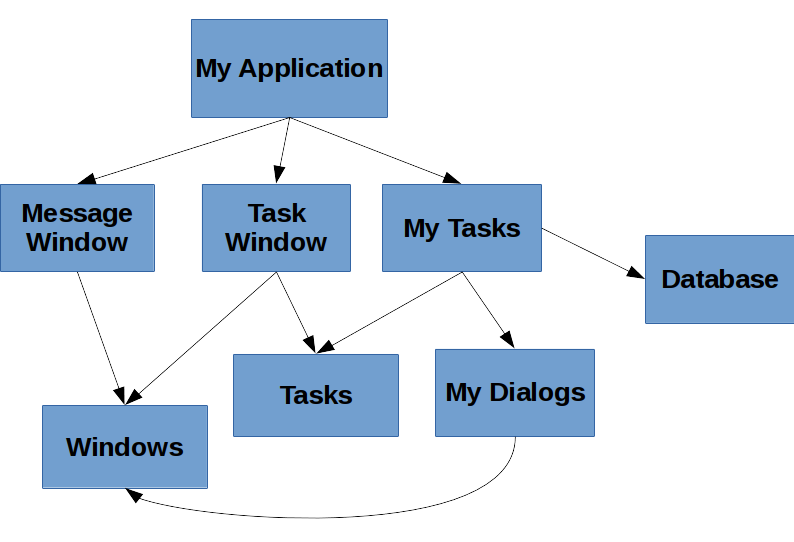
\includegraphics[width=\textwidth]{uml/DAG.png}
    \caption{Package Diagram are a Directed Acyclic Graph}
    \label{DAG}
\end{figure}

This structures has no cycles. It is a directed acyclic graph (DAG). 
When the team responsible for {\it My Dialogs} make a new release of 
their package, it is easy to find out who is affected. 
You just follow the dependency arrows backwards.
Thus, {\it My Tasks} and {\it My Application} are both goint to be affected.
The developers currently working on those packages will have to decide when 
they should integrate with new release of \textit{My Dialogs}.

Notice also that when \textit{My Dialogs} is released, it have no effect on
many other packages in the system. They don't know about \textit{My Dialogs}, and they don't care when it changes. This is nice. It mean that the impact
of releasing \textit{My Dialogs} is relatively small.

When the developers working on the \textit{My Dialogs} package would like 
to run a test of that package, all they need to do is compile and link their
version of \textit{My Dialogs} with the version of \textit{Windows} package
that they are currently using. None of the other packages in the system need
to be involved. 
This is nice; it mean that the developers working on \textit{My Dialogs} 
have relatively little work to do to set up a test, and there are 
relatively few variables for them to consider.

When it is time to release the whole system, it is done from bottom up. 
This process is very clear and easy to deal with. 
We know how to build the system because we understand the dependencies
between its parts.

\subsubsection{The Effect of a Cycle in the Package Dependency Graph}

Let assume that a new requirement forces use to change on of the classes
in \textit{My Dialogs} such that it makes use of a class in \textit{My Application}. This creates a dependency cycle as show in Figure \ref{NonDAG}.

\begin{figure}[H]
    \centering
    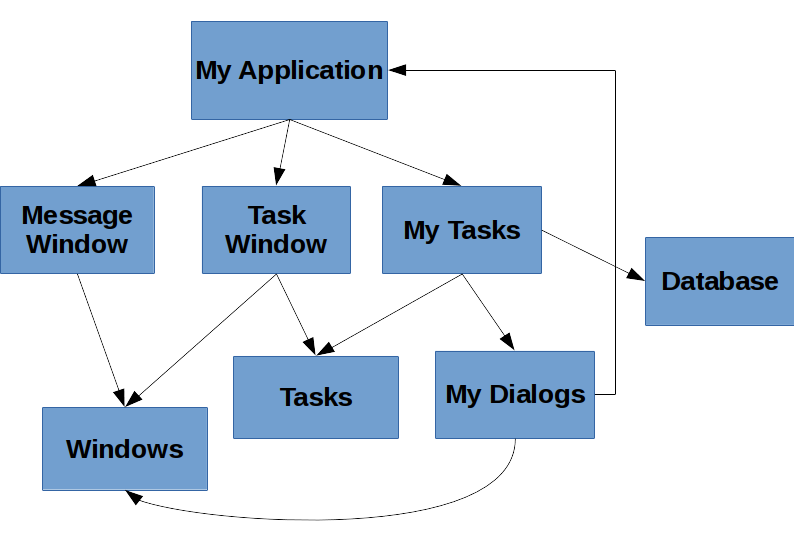
\includegraphics[width=\textwidth]{uml/NonDAG.png}
    \caption{A Package Diagram with a Cycle}
    \label{NonDAG}
\end{figure}

This cycle creates some immediate problems.
For example, the developers working on the \textit{My Tasks}
package know that in order to release, they must compatible with 
\textit{Task}, \textit{My Dialogs}, \textit{Database}, and 
\textit{Windows}. However, with the cycle in place, they must now also be 
compatible with \textit{My Application}, \textit{Task Window}, and 
\textit{Message Window}; that is the whole system.
This makes \textit{My Tasks} very difficult to release. 
All the developers who are working in one of those packages will 
experience the morning-after syndrome once again.

But this is just part of the trouble. Consider what happens when we want to test the \textit{My Dialogs} package. We find that we must link every other package in the system, including the \textit{Database} package.
This means that we have to do a complete build just to test 
\textit{My Dialogs}.
And in C++, compile grow geometrically with the number of modules.

Moreover, when there are cycles in the dependency graph, it can be very
difficult to work out the order in which to build the packages. There may be
no correct order.
This can lead to some very nasty problems in language like 
Java that read their declarations from compiled binary files.

\subsubsection{Breaking the Cycle}
It is always possible to break a cycle in package dependency graph.
There are two primary mechanism.

\begin{enumerate}
    \item Apply the Dependency-Inversion Principle (DIP). 
        (See Figure \ref{DIP})
    \item Create a new package on which both \textit{My Dialogs} and 
        \textit{My Application} depend. Move the class(es) that they 
        both depend on into that new package. 
        (See Figure \ref{new-package})
\end{enumerate}

\begin{figure}[H]
    \centering
    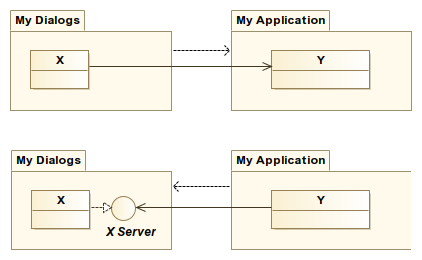
\includegraphics[width=10cm]{uml/DIP.png}
    \caption{Breaking the Cycle with a DIP}
    \label{DIP}
\end{figure}

\begin{figure}[H]
    \centering
    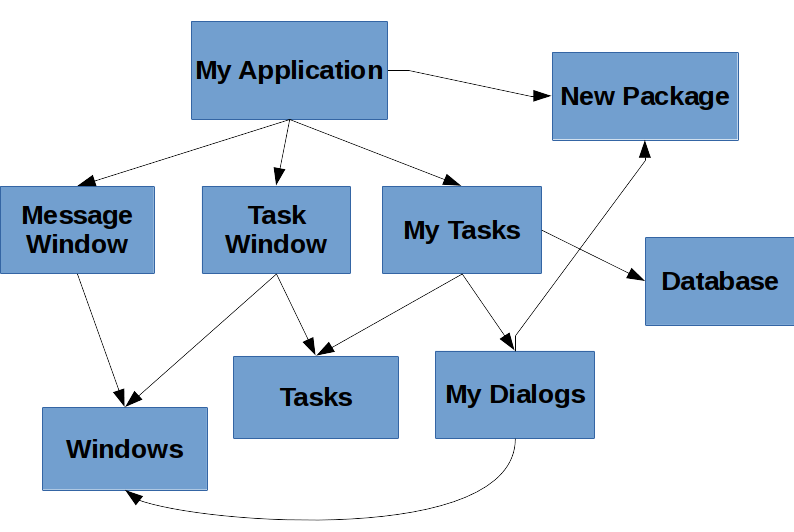
\includegraphics[width=\textwidth]{uml/new-package.png}
    \caption{Breaking the Cycle with a new package}
    \label{new-package}
\end{figure}

\subsubsection{Top-Down Design}
The package structure cannot be designed from top-down. This mean it is not one of the first things about the system that is designed. 
It seems that it evolves as the system grows and changes. 

You may find this to be counterintuitive. 
We have come to expect that large-grained decompositions, 
like packages, are also high-level functional decompositions. 
When we see a large-grained grouping like a package
dependency structure, 
we feel that the packages ought to somehow represent the functions 
of the system. Yet this does not seem to be an attribute of package dependency diagrams.

In fact, package dependency diagrams have very little 
to do with describing the function of the application.
Instead, they are a map to the buildability of the application. 
This is why they aren't designed at the start of the project. 
There is no software to build, and so there is no need for a build map. 
But as more and more classes accumulate in the 
early stages of implementation and design, 
there is a growing need to manage the dependencies so that 
the project can be developed without the morning-after syndrome. 
Moreover, we want to keep changes as localized as possible, 
so we start paying attention to the SRP and CCP and 
allocate classes that are likely to change together.

As the application continues to grow, 
we start becoming concerned about creating reusable elements. 
Thus, the CRP begins to dictate the composition of the packages. 
Finally, as cycles appear, the ADP is applied to break the cycles.

\subsection{The Stable-Dependencies Principle (SDP)}

\tab \textit{Depend in the direction of stability.}

Design cannot be completely static. Some volatility is necessary if the
design is to be maintained. We accomplish this by comforming to the 
Common-Closure Principle. Using this principle, we created packages that are
sensitive to certain kinds of changes. These packages are designed to be
volatile. We expect them to change. 

Any package that we expect to be volatile 
should not be depended on a package 
that is difficult to change. Otherwise, the volatile package will also be 
difficult to change. A module that you have designed to be easy to change 
can be made hard to change by someone else simply hanging a dependency 
on it. By comforming to the SDP, we ensure that the modules that are 
intended to be easy to change are not depended on modules that are harder 
to change than they are. 

\subsubsection{Stability}

There are many factors that make a software package hard 
to change: its size, complexity, clarity, etc. 
We are going to ignore all those factors and focus on something different. 
One sure way to make a software package difficult to change is to 
make lots of other software packages depend on it. 
A package with  lots of incoming dependencies is very stable because 
it requires a great deal of work to make any changes with all the dependent
packages.

Figure \ref{Stable} shows X, a stable package. This package has three 
packages depending on it; and therefore, it has three good reasons 
not to change. We say that it is responsible to those three packages. 
On the other hand, x depends on nothing, 
so it has no external influence to make it change. 
We say it is independent.

\begin{figure}[H]
    \centering
    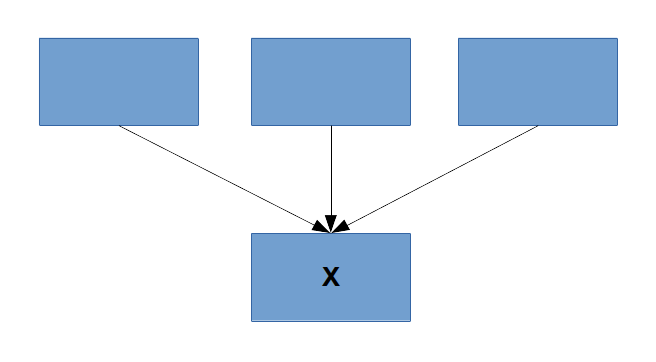
\includegraphics[width=10cm]{uml/Stable.png}
    \caption{X: A stable package}
    \label{Stable}
\end{figure}

In Figure \ref{Instable} on the other hand, shows a very instable package. 
Y have no other packages depending on it; we say that is is irresponsible.
Y also has three packages that it depends on, so changes may come from 
three external sources. We say that Y is dependent.

\begin{figure}[H]
    \centering
    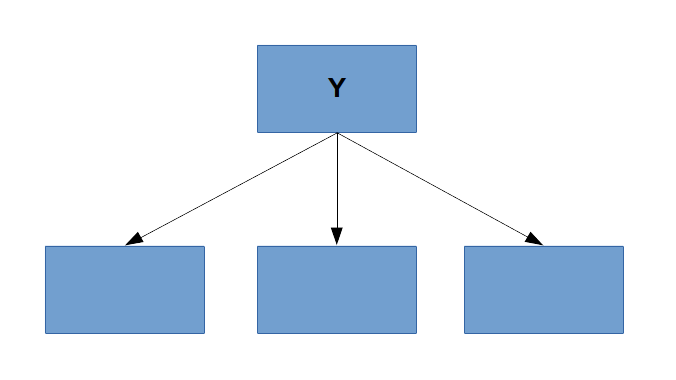
\includegraphics[width=10cm]{uml/Instable.png}
    \caption{Y: A instable package}
    \label{Instable}
\end{figure}

\subsubsection{Not All Packages Should Be Stable}
If all the packges in a system were maximally stable, the system would 
be unchangeable. This is not a desirable situation. 
We want to design our package structure so that some packages are instable 
and some are stable. And the stable packages should not 
depend on instable package. 

Figure \ref{ViolateSDP} show how the SDP can be violated. 
Flexible is a package that we intend to be easy to change. 
We want \textit{Flexible} to be instable. However some developer working in the 
package named \textit{Stable}, make a dependency on \textit{Flexible}. 
This violates the SDP since a stable package depend on an instable package.
As a result, \textit{Flexible} will no longer be easy to change. 
A change to \textit{Flexible} will force us to deal with \textit{Stable} and all its dependents.

\begin{figure}[H]
    \centering
    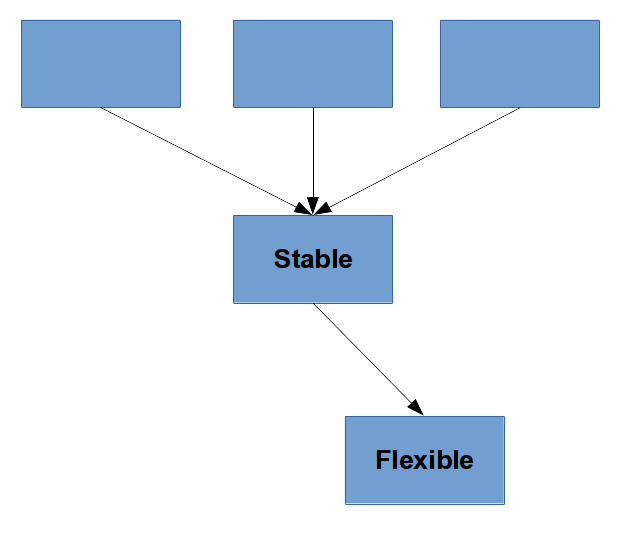
\includegraphics[width=10cm]{uml/ViolateSDP.png}
    \caption{Violation of SDP}
    \label{ViolateSDP}
\end{figure}

\begin{figure}[H]
    \centering
    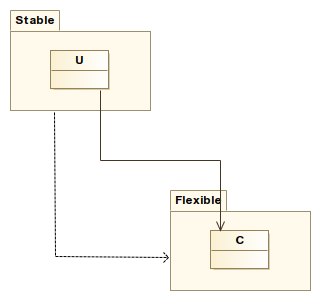
\includegraphics[width=8cm]{uml/cause-of-violation.png}
    \caption{Cause of violation of SDP}
    \label{CauseOfViolation}
\end{figure}

We can fix this by using the DIP. We create an interface called \textit{IU} and put it in a package named \textit{UInterface}. We make sure that this 
interface declares all the methods that U needs to use.
We make C inherits from this interface. This breaks dependency of 
\textit{Stable} on \textit{Flexible} and forces both packages to 
be dependent on \textit{UInterface}. (See Figure \ref{FixUsingSDP})

\begin{figure}[H]
    \centering
    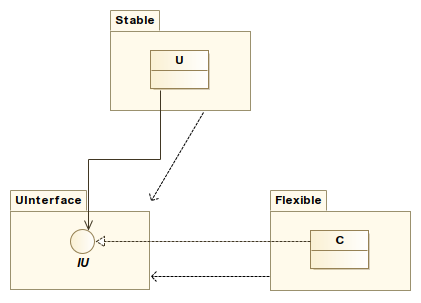
\includegraphics[width=8cm]{uml/fix-using-dip.png}
    \caption{Fixing the violation of SDP using DIP}
    \label{FixUsingSDP}
\end{figure}


\subsection{The Stable-Abstraction Principle (SAP)}

\tab \textit{A package should be as abstract as it is stable.} \cite{agile}

This principle sets up a relationship between 
stability and abstractness. It says that a stable package should also be
abstract so that its stability does not prevent it from being extended. 
On the other hand, it says that an instable
package should be concrete since its instability 
allows the concrete code within it to be easily changed.

Thus, if a package is to be stable, it should also consist of 
abstract classes so that it can be extended. 
Stable packages that are extensible are flexible and do not make many  
constrains for the design.

The SAP and the SDP combined amount to the DIP for packages. 
This is true because the SDP says that dependencies should run in direction
of stability, and the SAP says that stability implies abstraction. Thus, 
dependencies run in the direction of abstraction. 


\bibliography{report}{}
\bibliographystyle{plain}

\end{document}
